\subsection{Pengujian Deteksi Pose}
\label{subsec:posedetectiontesting}

\begin{figure} [ht]
  \centering
  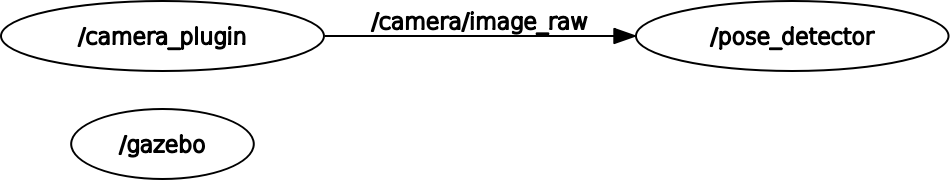
\includegraphics[width=0.45\textwidth]{figures/rosgraph/pose-detection.png}
  \IfLanguageName{english}{
    \caption{Node scheme of the pose detection testing.}
  }{
    \caption{Skema \emph{node} dari pengujian deteksi pose.}
  }
  \label{fig:rosgraphposedetection}
\end{figure}


Pengujian deteksi pose dilakukan di simulasi dengan tujuan untuk menguji kemampuan model pengguna dalam mensimulasikan pengguna \emph{real}.
Pada pengujian ini,
  \emph{node} \lstinline{pose_detector} akan dijalankan untuk melakukan proses visi komputer dalam mendeteksi pose pengguna.
Seperti yang terlihat pada gambar \ref{fig:rosgraphposedetection},
  \emph{node} \lstinline{pose_detector} akan terhubung dengan \emph{node} \lstinline{camera_plugin} yang akan mengirimkan data citra pengguna yang kemudian akan diolah oleh \emph{node} \lstinline{pose detector} untuk menghasilkan pose yang terdeteksi.

\begin{figure} [ht]
  \centering
  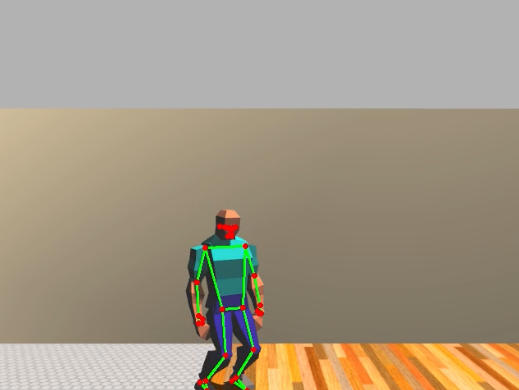
\includegraphics[width=0.4\textwidth]{figures/pose-detection.png}
  \IfLanguageName{english}{
    \caption{User pose detection results.}
  }{
    \caption{Hasil deteksi pose pengguna.}
  }
  \label{fig:posedetection}
\end{figure}


Hasilnya,
  seperti yang terlihat pada gambar \ref{fig:posedetection},
  dari citra yang diterima,
  \emph{node} \lstinline{pose_detector} akan mendeteksi pose dari pengguna tersebut dan menampilkan hasilnya sebagai garis dan titik pada citra yang diterima.
Selain itu,
  deteksi pose juga mampu menampilkan hasil yang sesuai ketika postur pengguna diubah dari berdiri ke duduk seperti hasil gambar \ref{fig:posedetection} tersebut.
